% =========================================================================
% CVPR 2027 draft — "Any Sensor In, Procedural Plant Out"
% -------------------------------------------------------------------------
% TEMPLATE NOTE: drafted under article.cls so it compiles anywhere.
% For submission, switch to the official CVPR 2027 kit:
%   \documentclass[10pt,twocolumn,letterpaper]{article} + \usepackage{cvpr}
% and replace \bibliographystyle{unsrtnat} with ieee_fullname.
% -------------------------------------------------------------------------
% NUMBERS: all quantitative results below are from the 15K-plant
% Sorghum/Maize studies (progress review, Oct 1 2026). Refresh every
% \oldnum{} value from the 10K--100K reruns before submission.
% =========================================================================
\documentclass[10pt,twocolumn,letterpaper]{article}

%%%%%%%%% PAPER TYPE  - PLEASE UPDATE FOR FINAL VERSION
% \usepackage{cvpr}              % To produce the CAMERA-READY version
\usepackage[review]{cvpr}      % To produce the REVIEW version
% \usepackage[pagenumbers]{cvpr} % To force page numbers, e.g. for an arXiv version

% Import additional packages in the preamble file, before hyperref
%% This file contains a number of tweaks that are typically applied to the main document.
%% They are not enabled by default, but can be enabled by uncommenting the relevant lines.

%%
%% Inline annotations; for predefined colors, refer to "dvipsnames" in the xcolor package:
%% https://tinyurl.com/overleaf-colors
%%
\newcommand{\red}[1]{{\color{red}#1}}
\newcommand{\todo}[1]{{\color{red}#1}}
\newcommand{\TODO}[1]{\textbf{\color{red}[TODO: #1]}}
%%
%% disable for camera ready / submission by uncommenting these lines  
%%
% \renewcommand{\TODO}[1]{}
% \renewcommand{\todo}[1]{#1}

%%
%% work harder in optimizing text layout. Typically shrinks text by 1/6 of page, enable
%% it at the very end of the writing process, when you are just above the page limit
%%
% \usepackage{microtype}

%%
%% fine-tune paragraph spacing
%%
% \renewcommand{\paragraph}[1]{\vspace{.5em}\noindent\textbf{#1.}}

%%
%% globally adjusts space between figure and caption
%%
% \setlength{\abovecaptionskip}{.5em}


%%
%% Allows "the use of \paper to refer to the project name"
%% with automatic management of space at the end of the word
%%
% \usepackage{xspace}
% \newcommand{\paper}{ProjectName\xspace}

%%
%% Commonly used math definitions
%%
% \DeclareMathOperator*{\argmin}{arg\,min}
% \DeclareMathOperator*{\argmax}{arg\,max}

%%
%% Tigthen underline
%%
% \usepackage{soul}
% \setuldepth{foobar}

% It is strongly recommended to use hyperref, especially for the review version.
% hyperref with option pagebackref eases the reviewers' job.
% Please disable hyperref *only* if you encounter grave issues, 
% e.g. with the file validation for the camera-ready version.
%
% If you comment hyperref and then uncomment it, you should delete *.aux before re-running LaTeX.
% (Or just hit 'q' on the first LaTeX run, let it finish, and you should be clear).
\definecolor{cvprblue}{rgb}{0.21,0.49,0.74}
\usepackage[pagebackref,breaklinks,colorlinks,allcolors=cvprblue]{hyperref}

% ---- draft machinery (delete before submission) -------------------------
% \newcommand{\todo}[1]{\textcolor{red}{[TODO: #1]}}
\newcommand{\oldnum}[1]{\textcolor{purple}{#1}} % number from 15K study; refresh
% ---- method name: placeholder. Candidates: CropCode, PhytoCode, FieldCode,
%      Canopy2Code. Decide with co-authors. ------------------------------
\newcommand{\method}{\textsc{CropCode}}
% ---- dataset name: placeholder. Candidates: FieldProc, ProcField3D,
%      CropForge, SlenderField. Named datasets get cited; decide early. --
\newcommand{\dataset}{\textsc{FieldProc}}
\newcommand{\cmark}{\checkmark}
\newcommand{\xmark}{$\times$}
\providecommand{\CropCode}{\textsc{CropCode}}
\providecommand{\FieldProc}{\textsc{FieldProc}}
\providecommand{\todo}[1]{\textcolor{red}{#1}}
\providecommand{\R}{\mathbb{R}}


%%%%%%%%% PAPER ID  - PLEASE UPDATE
\def\paperID{*****} % *** Enter the Paper ID here
\def\confName{CVPR}
\def\confYear{2027}

\usepackage{xcolor}
% \usepackage[colorlinks=true,linkcolor=blue,citecolor=blue,urlcolor=blue]{hyperref}


% ---- Title. Alternative (direction #4, maximal sobriety):
\title{Procedural Reconstruction of Slender Plants from Any Field Modality}
%\title{Any Sensor In, Procedural Plant Out:\\Occlusion-Robust Reconstruction of Slender Crops in the Field}

% CVPR is double blind — authors commented out for submission.
% \author{Anonymous CVPR 2027 submission}
\author{\todo{author block (ISU + Purdue); anonymize for submission}}
\date{}

\begin{document}

\maketitle

\begin{abstract}
Editable, biologically interpretable 3D models of field-grown crops
support high-throughput phenotyping, \emph{in silico} breeding trials,
and agronomic digital twins, but recovering such models from field
sensor data remains difficult: plant organs are slender, neighboring
plants occlude one another, and a field campaign rarely yields more than
a single photograph, a noisy depth frame, or a partial point cloud per
plant.
% (fix 2: vision hook — delete the next sentence if unwanted)
Slender geometry under occlusion is a regime in which learned 3D
completion and Chamfer-based evaluation both fail. In this work, we
present \method{}, a multimodal
masked-autoencoder framework that recovers the complete procedural
representation of a plant, the generator parameters encoding leaf
count, insertion heights, blade angles, and surface geometry, from any
subset of RGB, depth, and point-cloud input in a single forward pass.
The model is pretrained on \todo{10K--100K} procedurally generated maize
and sorghum plants rendered with physically simulated row occlusion, and
a full-modality teacher is then distilled into single-sensor students.
Distillation improves cross-modal generation by \oldnum{19\%} on average
and parameter recovery from a point cloud alone by \oldnum{44\%}.
Controlled ablations, replicated across both species, show that the
procedural parameters are valuable prediction targets but do not help
as a pretraining modality: exposing them to the encoder degrades
phenotype recovery on every sorghum target and does not improve it in maize. We further show that Chamfer distance and linear probes on
the frozen representation rank input modalities differently on slender
geometry, and we adopt the probe as the deciding metric. On real field
scans with independently reconstructed ground truth, \method{}
\todo{matches/approaches} the accuracy of a staged annotation pipeline
and reduces the time required for procedural reconstruction from hours of manual
specification, or minutes of pipeline computation, to milliseconds per
plant. We will release \dataset{}, the \todo{N}-plant, two-species benchmark
behind these experiments, which pairs multimodal field captures under
simulated row occlusion with exact procedural ground truth.
\end{abstract}    
\section{Introduction}
\label{sec:intro}

% ---- Fig. 1: teaser. TOP ROW: single RGB image -> \method{} ->
% predicted parameters -> editable 3D plant, INCLUDING one edit demo
% (change leaf angle, re-render) — immediately distinguishes this from
% point-cloud completion. BOTTOM STRIP: the difficulty progression,
% isolated -> self-occluded -> neighbor-occluded, with the other input
% modalities (depth / partial PCD) shown as alternative entry points.
% Downstream uses (simulation, trait analytics, compact storage) as
% small icons.
\begin{figure}[t]
  \centering
  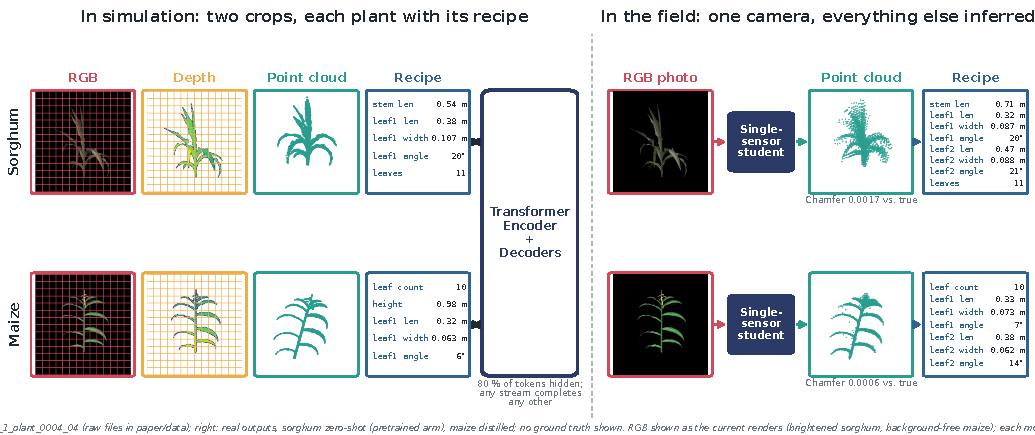
\includegraphics[width=\linewidth]{Figures/fig_teaser.pdf}
  \caption{\textbf{Any sensor in, procedural plant out.} From any subset
  of field-practical modalities (a single photograph, a depth frame, or
  a point cloud truncated by row neighbors), \method{} recovers the full
  procedural representation of the plant: a kilobyte-scale, physiologically
  interpretable parameter set that can be re-rendered to complete geometry,
  used as simulation input, and used for trait analytics at field scale.
  \todo{replace box with figure}}
  \label{fig:teaser}
\end{figure}

% P1 — Goal. (GPS: goal)
Accurate three-dimensional models of individual crop plants enable
high-throughput phenotyping of morphological traits such as leaf angle,
internode length, and canopy architecture, and they are the basis of emerging
agricultural digital twins in which breeding trials run \emph{in
silico}~\citep{hadadi2025procedural, maizefield3d2025}. The representation
best suited to these uses is procedural: a compact set of biologically
interpretable parameters that a generator expands into complete,
editable, simulation-ready geometry~\citep{prusin1990abop,
floraforge2026}. A procedural plant occupies a few kilobytes where a
laser scan occupies megabytes, every parameter corresponds to a trait used by
agronomists, and the model can be edited, re-rendered, and
perturbed in ways that unstructured geometry does not support.
% (fix 2: vision hook — delete the next sentence if unwanted)
Field crops also instantiate a challenge of general interest in 3D
computer vision: recovering a parametric model of a thin, heavily
occluded object from partial multimodal observations.

% P2 — Problem, part 1: existing routes presuppose a rich input. (GPS: problem)
Yet recovering procedural structure from field-acquired sensor data
remains a significant challenge, and every existing route presupposes a
rich, clean observation. Manual parameter specification takes hours per
plant~\citep{floraforge2026}. Staged reconstruction pipelines automate
the process; a recent system annotates laser scans with a
vision-language model and fits a procedural descriptor to
\oldnum{5.4}\,mm median accuracy, but it requires a complete scan of an
isolated plant and roughly ten minutes of computation per
plant~\citep{hadadi2026vlmmaize}. Per-scene optimization methods search
generator parameters against multi-view imagery~\citep{cropcraft2026},
and recent learned models infer parametric plants, but only
from a clean, complete point cloud~\citep{demeter2025,
ghrer2025paramplants}. A phenotyping campaign produces the opposite:
thousands of plants per day, each observed by whichever sensor was
practical (a camera, a depth frame, or a partial scan).

% P3 — Problem, part 2: the geometric frontier. (GPS: problem, sharpened)
In addition, crop plants
are slender: a maize blade is centimeters wide, millimeters thick, and
up to a meter long. In a planted row, each plant is further occluded by
its neighbors, whose leaves interleave with the target; in our field
simulations, roughly a third of the points inside a plant's bounding
region belong to neighboring plants. This regime violates the
assumptions of learned 3D completion: the standard benchmarks contain
compact, largely convex objects and no slender-under-occlusion
category~\citep{yuan2018pcn,yu2021pointr}, and Chamfer distance, the
default metric, is structurally insensitive to thin sheets, so it can
reward reconstructions that miss entire blades~\citep{wu2021dcd,
song2026structural}. Occlusion-aware completion of thin plant organs has begun to address
the input side of this regime, but its output is a completed point
cloud rather than structure~\citep{lee2026occ}.
% TODO-bib: add thinleaf_completion2024 (Plant Phenomics 2024) and
% cornleaf_gridding2023 (Remote Sensing 2023) to CVPR.bib and cite here.
To our knowledge, no prior method recovers a procedural, re-renderable
representation of slender crop organs from a single field-practical
observation (a photograph, a depth frame, or a partial point cloud)
under row-neighbor occlusion: methods that infer plant
parameters require clean, complete scans of isolated
plants~\citep{demeter2025,ghrer2025paramplants}, and methods that
tolerate field occlusion complete unstructured geometry
instead~\citep{lee2026occ}.

% P4 — Solution: the framework. (GPS: solution)
In this work, we present \method{}, a framework that makes this inverse
problem tractable by using the procedural generator itself as the prior.
We pretrain a four-stream masked
autoencoder~\citep{he2022mae,bachmann2022multimae,mizrahi2023fourm,
dong2025embodiedmae} over RGB, depth, point clouds, and tokenized
procedural parameters of \todo{10K--100K} generated maize and sorghum
plants, rendered in simulated rows in which neighboring leaves bend on
contact. Because random modality subsets are masked during pretraining,
a single model learns to complete any subset at inference. A
full-modality teacher is then distilled~\citep{hinton2015distillation}
into single-sensor students for deployment. Distillation
improves cross-modal generation by \oldnum{19.1\%} on average and by
\oldnum{27.5\%} when conditioning on a point cloud alone, and it improves
parameter recovery from that point cloud by \oldnum{43.8\%}.

% P5 — Finding 1: parameters belong at the output.
We also address a design question that arises for any model with access
to generative structure: where should the parameter stream enter? In our
controlled ablations, the parameters are valuable prediction targets but
harm the representation when used as an encoder input. With token budgets
matched, adding the parameter stream to the encoder degrades the frozen
representation on every sorghum phenotype target, and on maize the paired
comparison is a draw. In sorghum, the loss persists in control arms that
restore the sensor-token budget, and it persists even when the parameters
serve only as a reconstruction target for the decoder. Supervising
parameters as a generation target, however, lets the distilled generalist
outperform a parameter-only specialist at parameter regression. One
interpretation, consistent with modality competition~\citep{peng2022ogm}
and negative transfer~\citep{yu2020pcgrad}, is that a stream that already
contains the answer suppresses learning in the streams that must provide the
trait information at test time.

% P6 — Finding 2: metrics.
Chamfer distance ranks depth as the most valuable input
modality (\oldnum{$-32\%$}), whereas a linear probe on the frozen
representation, read out on phenotypic traits, ranks depth within noise
and identifies RGB as the main source of trait information. On slender geometry the two metrics measure
different quantities, surface proximity and recovered structure, and we
adopt the probe as the deciding metric for modality
decisions~\citep{chen2020simclr,wu2021dcd}.

% P7 — Claim + validation + contributions.
We claim that fragmentary field sensing suffices to
recover a complete, interpretable procedural plant, provided the
generator is used for both the training data and the output
representation. We
validate this claim on real field
scans of maize and sorghum with independently reconstructed ground
truth~\citep{maizefield3d2025,hadadi2026vlmmaize}, including rows in
which neighbors occlude the target.
\todo{one sentence of headline real-data results when available.}
The key contributions of this work are:
\begin{enumerate}
  \item \textbf{Task and framework.} The first formulation and system, to
  our knowledge, for recovering procedural plant representations of
  slender, row-occluded field crops from \emph{any subset} of RGB, depth,
  and point-cloud input in one amortized forward pass, with full-modal to
  single-sensor distillation (+\oldnum{19.1\%} generation,
  $-$\oldnum{43.8\%} parameter error from point clouds alone).
  \item \textbf{A design rule for structured modalities.} Controlled,
  budget-matched, two-species evidence that generator parameters are
  valuable prediction targets, while treating them as an auxiliary
  representation-learning modality does not improve, and can degrade,
  the sensor representation; we expect this guidance to transfer to any
  multimodal model with access to privileged generative structure.
  \item \textbf{An evaluation protocol for slender geometry.} A
  demonstration that Chamfer distance and downstream phenotype probes
  disagree systematically on slender organs, and a frozen-latent probe
  protocol that resolves modality decisions where Chamfer is insensitive.
  \item \textbf{A benchmark.} \dataset{}, a two-species procedural
  field benchmark of \todo{N} plants spanning \todo{diversity axes:
  phenotypes / generator configurations / occlusion severities}, with
  paired multimodal captures, physically simulated row occlusion, and
  exact parameter ground truth, together with a real-field evaluation
  split carrying reconstructed procedural ground truth across the
  genotypes of a diversity panel~\citep{maizefield3d2025}. No existing
  dataset combines these elements
  (Tab.~\ref{tab:datacompare})~\citep{schunck2021pheno4d,yuan2018pcn}.
  We will release the data, generation code, and evaluation scripts.
  \todo{confirm release scope and licensing}
\end{enumerate}

\section{Related Work}
\label{sec:related}
% Compressed from Appendix A. One paragraph per thread; each opens with
% the claim, closes with the differentiation.

\paragraph{Recovering procedural plants.}
Inverse procedural modeling has a long history for woody plants:
parameters of tree generators have been recovered by stochastic
search~\citep{stava2014ipmtrees}, by Markov chain Monte Carlo
inference~\citep{talton2011metropolis}, and by inferring L-systems
directly from point clouds~\citep{guo2020ipmlsys,latentlsys2023}. These
methods optimize or infer per instance. Recent systems address crops
specifically. Demeter learns a parametric morphology model from soybean
point clouds~\citep{demeter2025}, Ghrer et al.\ infer grammar-style
plant representations from 3D scans~\citep{ghrer2025paramplants},
CropCraft fits a procedural crop model by Bayesian optimization against
multi-view imagery~\citep{cropcraft2026}, and a recent staged pipeline
reconstructs procedural maize from terrestrial laser scans through
vision-language-model annotation and differentiable NURBS
refinement~\citep{hadadi2026vlmmaize,nurbsdiff2022}. Each of these
methods presupposes a single rich observation, a clean and complete
point cloud or a multi-view capture of an isolated plant, and none
addresses missing modalities or inter-plant occlusion.

\paragraph{Programs from observations.}
Outside agriculture, decoding parametric programs from observations is
an established pattern: neural shape programs~\citep{shapeprograms2019},
diffusion-based inverse procedural content generation from a single
image~\citep{zhao2025dipcg}, text-conditioned CAD
generation~\citep{text2cad2024}, and cadrille, which maps images, point
clouds, or text to executable CAD models~\citep{kolodiazhnyi2025cadrille}.
These systems operate on rigid objects observed cleanly and in
isolation. Our setting differs in the geometry (deformable, slender
organs), in the input (noisy, occluded field sensors), and in a design
question that none of them raises: whether the program parameters
should be visible to the encoder at all.

\paragraph{Completion and slender geometry.}
Learned point cloud completion has progressed from folding-based
decoders~\citep{yuan2018pcn} to geometry-aware
transformers~\citep{yu2021pointr,yu2023adapointr,cai2024einet}, trained
on benchmarks of compact, largely convex objects that contain no
slender-under-occlusion category. Completion of thin plant organs under
occlusion has emerged recently~\citep{lee2026occ}, and reconstruction
of thin structures from clean multi-view data is an active
topic~\citep{curvegaussian2025,qi2026rethinking}, but in both lines the
output is unstructured geometry rather than an editable model. Chamfer
distance, the standard completion metric, is insensitive to thin sheets
and can be reduced by collapsing predictions onto bulk
structure~\citep{wu2021dcd,song2026structural,lin2023infocd}; we therefore
evaluate with trait probes alongside geometric metrics
(Sec.~\ref{sec:exp-metrics}).

\paragraph{Multimodal masked pretraining.}
Masked autoencoding~\citep{he2022mae} extends to multiple modalities in
MultiMAE~\citep{bachmann2022multimae}, to any-to-any generation over
tokenized modalities in 4M~\citep{mizrahi2023fourm,bachmann2024fourm21},
to point clouds in Point-MAE~\citep{pang2022pointmae}, and to combined
RGB, depth, and point cloud inputs in EmbodiedMAE, from which our
architecture derives~\citep{dong2025embodiedmae}. Robustness to missing
modalities is a recognized concern~\citep{wang2024robustmissing}, and
distillation from multi-sensor teachers to single-sensor students is
established for discriminative tasks~\citep{hinton2015distillation}. We
extend this machinery in two ways: we add a structured generative
modality, encoded with continuous number tokens~\citep{golkar2023xval},
and we distill a generative full-modality teacher for structured
parameter regression.

\paragraph{Learning from procedural data.}
Pretraining on purely synthetic data is viable, from abstract
fractals~\citep{kataoka2020fractaldb} to procedurally generated
scenes~\citep{raistrick2023infinigen,greff2022kubric}, with domain
randomization bridging the gap to real
data~\citep{tobin2017domainrand} and with the value of synthetic data
known to depend on the downstream task~\citep{fan2023intriguing}. Our
setting is the favorable case for this strategy: the procedural
generator defines the output representation, spans the morphology of
the target crop, and is paired with real field evaluation
data~\citep{maizefield3d2025}. Our results add one caveat to the
recipe: the generator's parameters are valuable as data and as targets,
but exposing them to the encoder costs representation quality
(Sec.~\ref{sec:exp-params}).


% =========================================================================
\section{Method}
\label{sec:method}

In this section, we present \CropCode{}, a multimodal framework for recovering
procedural plant representations from incomplete sensor observations. We first
formulate the reconstruction task and describe the procedural data generation
process. Next, we introduce the token representations and masked pretraining
objective. Finally, we describe the teacher--student training strategy for
single-sensor inference and the protocol used to evaluate transfer to field
observations. An overview of the framework is shown in Fig.~\ref{fig:arch}.


% ---- FIG 2 (architecture, full width): four token streams entering a
% shared encoder (RGB patches / depth patches / PC groups / xVal param
% tokens), Dirichlet mask sampler on top, four decoders out; a second
% panel showing teacher (all streams) -> distill -> student (one stream).
\begin{figure*}[t]
  \centering
  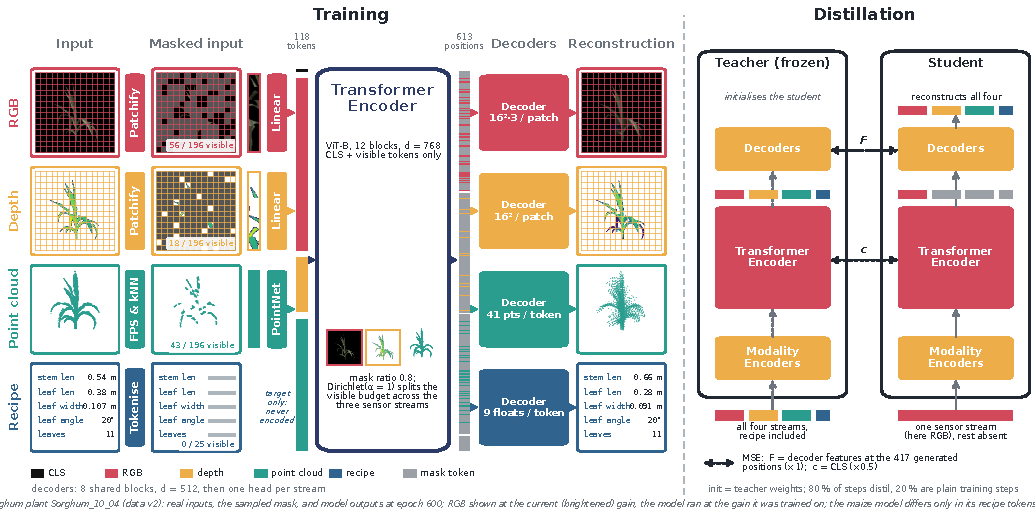
\includegraphics[width=\linewidth]{Figures/fig_architecture.pdf}
  \caption{\textbf{\method{} overview.} (a) Four token streams enter a
  shared encoder under a Dirichlet masking budget; modality-specific
  decoders reconstruct all streams. During pretraining the parameter
  stream is both masked input and decoder target; its role is ablated in
  Sec.~\ref{sec:exp-params}. (b) The full-modality
  teacher is distilled into single-sensor students for deployment.}
  \label{fig:arch}
\end{figure*}

\subsection{Problem formulation}
\label{sec:method-form}
% Talking points:
% - A plant is a program: theta in R^d (plant-level + per-leaf fields;
%   d ~ \todo{X} for maize, \todo{Y} for sorghum), generator G(theta) ->
%   mesh -> any sensor rendering.
% - Observation: O = any nonempty subset of {I_rgb, I_depth, P_partial},
%   degraded by view sparsity, sensor noise, and ROW OCCLUSION (neighbor
%   points inside the target's region, bent-leaf contact geometry).
% - Task: a single amortized f(O) -> (theta_hat, I_rgb, I_depth, P_full):
%   procedural parameters PLUS completed modalities, one forward pass.
% - State the well-posedness argument: slender+occluded geometry is
%   underdetermined; G's parameterization is the prior that closes it.
\todo{3 short paragraphs from the bullets}

Let $G$ denote a procedural generator that maps a parameter vector
$\theta\in\R^{d_\theta}$ to a plant mesh $G(\theta)$. The parameters describe
plant-level structure, including stem and panicle geometry, together with
leaf-level attributes such as insertion height, length, roll, branching angle,
and blade width. We consider three sensor modalities,
$\mathcal{M}=\{\mathrm{rgb},\mathrm{d},\mathrm{pc}\}$, corresponding to an RGB
image, a depth frame, and a point cloud. In field conditions, only a subset
$S\subseteq\mathcal{M}$ may be available, and each observation may contain
partial geometry or occlusion from neighboring plants. Our objective is to
recover the underlying procedural representation from these observations.

We formulate this task as feed-forward prediction:
\begin{equation}
  f_\phi\!\left(\{x^m:m\in S\}\right)
  = \left(\hat\theta,\{\hat x^m:m\in\mathcal{M}\}\right),
  \label{eq:procedural-inverse}
\end{equation}
where $\phi$ denotes the network parameters, $\hat\theta$ is the predicted
plant description, and $\hat x^m$ denotes the reconstructed sensor modalities.
The procedural output $G(\hat\theta)$ supports geometric reconstruction and
trait analysis within the same representation. Unlike per-instance fitting
of a procedural model to a scan~\cite{hadadi2026vlmmaize}, this formulation
learns a shared inverse mapping that is applied to each new observation in a
single forward pass.

The procedural generator provides both the training observations and their
exact parameter targets. This allows us to supervise parameter recovery
without manually annotating each synthetic plant. At deployment, however,
$\theta$ is unknown and must be inferred exclusively from sensor input. We
therefore distinguish its role as a reconstruction target from its possible
use as privileged input during training. The visibility of the parameter
stream is controlled separately, allowing us to study this distinction while
keeping the sensor-token budget fixed (Sec.~\ref{sec:param-stream}).



\subsection{A procedural field-data engine}
\label{sec:method-data}

\begin{table}[t]
  \centering\small
  \setlength{\tabcolsep}{3pt}
  \begin{tabular}{lcc}
    \toprule
     & Maize & Sorghum \\
    \midrule
    Plants & 15{,}000 & 15{,}000 \\
    Split (train/val/test) & \multicolumn{2}{c}{10{,}500 / 2{,}250 / 2{,}250} \\
    Views per plant & 10, random & 10, fixed rig \\
    Camera distance & fitted per plant & 2.5\,m \\
    Per-view cloud & 8{,}192 pts, visible & complete \\
    Parameter slots ($d_\theta$) & $14+14\times28$ & $9+5\times24$ \\
    Leaf count range & \todo{3--22} & 4--35 \\
    Plant height & 0.62--1.44\,m & stem 0.19--1.74\,m \\
    Rows $\times$ orientations & $15{,}000\times10$ & $15{,}000\times10$ \\
    Row camera & level, 1.0\,m & level, 2.5\,m \\
    Row cloud in / target & \multicolumn{2}{c}{24{,}576 / 8{,}192 pts} \\
    Real-field split & \todo{MaizeField3D} & \todo{TBD} \\
    \bottomrule
  \end{tabular}
  \caption{\FieldProc{} dataset configuration. The parameter dimension
  includes plant-level attributes and a fixed number of leaf slots. Every
  row has one main plant from the split and two neighbours at a 0.15\,m
  stem spacing, widened only when the contact solver needs it
  (Supp.~\ref{app:data}). \todo{Confirm the maize leaf-count range and the
  real-data splits~\cite{maizefield3d2025}.}}
  \label{tab:fieldproc}
\end{table}

\paragraph{Procedural generation.}
We construct \FieldProc{} using species-specific generators for maize and
sorghum, 15{,}000 plants each. Plant $i$ is generated with random seed $i$ and
is paired with its exact procedural parameters. Maize traits are drawn from
Gaussians (e.g.\ height $0.83\pm0.10$\,m, leaf count $12.4\pm2.6$, leaf angle
$44^\circ\pm10^\circ$) coupled through four latent traits (vigour, slenderness,
posture, texture), with canopy-position curves and per-leaf jitter; the plants
are 0.62--1.44\,m tall. Sorghum plants come from the EvoEngine sorghum
generator, which draws the heading, stem tilt, leaf count and internode length
per plant and evaluates per-leaf curves for insertion point, length, width,
roll (alternating sides), branching angle and bending; they carry 4--35 leaves
(mean 19.5) on stems of 0.19--1.74\,m. The populations therefore span
continuous variations in morphology rather than discrete genotype classes,
and we evaluate phenotype representations through regression. The generators
also differ in their trait dependencies. In sorghum, stem length is the
internode length times the leaf count, so it is strongly coupled to leaf
count ($\text{stem length}=0.05\,n_{\text{leaves}}-0.001$, $R^2=0.988$),
whereas this association is weak in maize ($r=0.20$). We therefore evaluate
both species to examine whether the observed behavior extends beyond a single
generator's correlations.

\paragraph{Isolated-plant observations.}
For each plant, we render ten views with \texttt{pyrender} at $1024\times1024$
and a $40^\circ$ vertical field of view, each with an RGB image, a depth image
stored losslessly as a packed 32-bit value, and the camera pose. Three fixed
directional lights are aimed at the plant's bounding-box centre. Images are
rendered on a grey background; in the final release it is made transparent
and composited over black. The
two species are captured differently. Sorghum views follow one fixed
Fibonacci-sphere rig at 2.5\,m, five directions above and five below the
horizon (elevations $-64^\circ$ to $+64^\circ$), so every plant is seen from
the same ten directions, and the per-view cloud is the complete,
occlusion-free plant cloud expressed in the camera frame. Maize views are ten
directions drawn uniformly on the sphere per plant, at a distance fitted to
the plant's bounding box, with an extra light at the camera; the per-view
cloud is 8{,}192 points back-projected from that view's depth image, so it
holds only the surface the camera sees. At 2.5\,m the lens covers about
1.8\,m of height, so the top or base of the tallest sorghum plants can fall
outside the frame.

\paragraph{Row observations.}
The row sets place each plant of a split, as the \emph{main} plant, between two
neighbours from the same split (one row per plant), with 0.15\,m between stem
bases. Each row is rendered at ten orientations: the main plant is turned
about its stem by $0^\circ,10^\circ,\dots,90^\circ$ and each neighbour by the
same angle plus a uniform offset in $\pm15^\circ$; sorghum neighbours are also
tilted so their stems run parallel to the main stem. Before rendering, a
contact solver makes the three plants free of intersections while keeping
them close to their grown shapes: each leaf blade is a chain of 8\,cm
segments whose joints bend along circular arcs, so blades stay smooth, keep
their length and stay attached, while stems, sheaths and tassels stay rigid.
A leaf that would cross another plant bends by the smallest clearing angle at
the joint before the contact; neighbours give way first, and a main-plant leaf
bends only where a neighbour cannot move. Contacts are decided by exact
triangle--triangle tests, so leaves may touch but never intersect. When no
layout exists under the bend limits, the limits are loosened in stages and
then the spacing is widened; in maize, 76--79\,\% of orientations are solved at
0.15\,m and none needs more than 0.33\,m. A rover camera, level and aimed at
the main plant's bounding-box centre from 1.0\,m (maize) or 2.5\,m (sorghum),
takes one shot per orientation, rendered twice: the input with all three
plants (RGBA, depth, and a 24{,}576-point cloud of every visible plant) and the
ground truth with the main plant alone, in its bent shape, from the same
camera (8{,}192 points). The parameter record describes the grown plant, so
the target geometry departs from it only where the solver had to bend a
main-plant leaf.
Occlusion is measured per shot from the two depth maps (maize, 120 train
rows): the fraction of the main plant's own pixels hidden behind a neighbour is
9\,\% on average, 13\,\% at $0^\circ$, where the generator's single leaf plane
lies along the row, falling to 1\,\% at $90^\circ$ (90th percentile 17\,\%),
and the neighbours supply 59--68\,\% of the plant pixels in the frame and two
thirds of the input cloud. \todo{Same measures for the sorghum rows.}

\paragraph{Data partitioning.}
We partition plants into training, validation, and test sets in a 70/15/15
ratio by plant, so all views and rows of a main plant fall in one split, and
we bias the held-out sets toward unusual morphologies. For maize, each plant is
scored by its Mahalanobis distance~\cite{mahalanobis2018generalized} from the
median over 19 robustly standardized parameter features, and the most extreme
plants are dealt alternately to test and validation, a pure tail split. For
sorghum, the extremeness is the Mahalanobis distance from the mean over six
features (leaf count, stem length, mean and maximum leaf length, mean and
standard deviation of leaf roll), and the probability of being held out rises
steadily with its rank, from 0.3\,\% in the least extreme 5\,\% of plants to
70\,\% in the most extreme 5\,\%; validation and test share one distribution.
\todo{The sorghum selection rule is inferred from the released assignment;
confirm it against the script that wrote it.}
We report errors in native trait units alongside $R^2$, since the latter
depends on the target distribution of each split. In the ablations, an epoch
samples one view per training plant, with identical view draws across compared
models. Data-scaling experiments use nested subsets of plants, each retaining
all ten available views, and match the number of optimizer updates.
% Original split diagnostic: median extremeness is 2.03 on train and 2.76 on
% validation/test. Retain in the dataset supplement; define rank scaling.




% - Two generators, two species: FloraForge maize (BTx99 phenotype,
%   rebuildable-from-file parameters) \citep{floraforge2026}; EvoEngine
%   sorghum. Hidden-trait correlation structure (vigor, slenderness,
%   posture, texture).
% - Row simulation: neighbors at d=0.40m, contact-resolved leaf bending
%   (no interpenetration, arcs preserve length), rotation about stem.
% - Capture model: 10 views/plant, 1024^2 RGB + metric depth, 8,192-pt
%   per-view camera-frame clouds, 60K-pt whole-plant GT; crop-box inputs
%   retain ~1/3 contaminating neighbor points.
% - Scale: \todo{10K-100K} plants/species; 70/15/15 split by plant.
% - BIOLOGICALLY CONSTRAINED SAMPLING: correlated developmental traits
%   (height, leaf count, internode spacing, insertion locations) sampled
%   jointly from allometrically constrained distributions WITH NOISE —
%   correlated but never deterministic (target the maize regime,
%   r~0.2 height/leaf-count, NOT sorghum's r=0.994 coupling, which
%   collapses trait evaluation to rank 2). Report conditional spreads.
%   Estimate the allometry from measured maize data where possible.
% - PARAMETER GROUPING: plant-level/developmental (height, leaf count,
%   stem diameter, internodes, insertion locations) vs organ-level/shape
%   (length, width, insertion angle, azimuth, droop, curvature, twist).
%   Headline evaluation traits: height, leaf count, leaf angle, length,
%   width, azimuth; waviness/spline fields stay in the representation
%   but not in headline metrics.
% - PAIRED OBSERVATIONS: every plant rendered BOTH isolated AND inserted
%   into a row (same morphology, harder observation); row spacing swept
%   \todo{0.15-0.70 m}; per-sample occlusion severity recorded
%   continuously (visible pixel fraction, visible 3D-point fraction,
%   neighbor contamination, hidden-leaf fraction).
% - CAMERA PROTOCOL: explicit, evidence-based axes — elevation ladder
%   (the documented difficulty axis) and azimuth relative to the leaf
%   plane (distichous maize); small schematic figure.
% - BACKGROUND / SENSOR MODEL: \todo{if the real acquisition commits to
%   strobe + short exposure, frame the dark background as a deliberate
%   sim-to-real co-design and add the black-vs-randomized-background
%   ablation evaluated on real strobe images; current captures use 0.5
%   grey — verify acquisition plan before adopting}.
% - Close with: exact parameter GT for every sample — the supervision no
%   real capture can provide.
% \begin{table}[h]\centering\small
% \begin{tabular}{lcc}
% \toprule
%  & Maize & Sorghum \\
% \midrule
% Plants                     & \todo{N}        & \todo{N} \\
% Views / plant              & 10              & 10 \\
% Parameters / plant         & \todo{d}        & \todo{d} \\
% Leaf count range           & 3--22           & 11--27 \\
% Occluded-row variants      & \todo{...}      & \todo{...} \\
% Neighbor points in crop   & \todo{$\sim$30\%} & \todo{...} \\
% \bottomrule
% \end{tabular}
% \caption{\dataset{} at a glance. \todo{finalize; add diversity axes
% (phenotypes / generator configs / growth stages) and real-data eval row
% (MaizeField3D scans + pipeline GT \citep{maizefield3d2025,
% hadadi2026vlmmaize})}}
% \label{tab:data}
% \end{table}



% ---- The "only row with all checkmarks" exhibit. Verified by the lit
% review: no existing dataset combines these properties.
\begin{table*}[h]\centering\small
\begin{tabular}{lcccccc}
\toprule
 & Real & Slender & Row occl. & RGB+D+PC & Proc.\ GT & Scale \\
\midrule
PCN / ShapeNet-55~\citep{yuan2018pcn,yu2021pointr}
          & \xmark & \xmark & \xmark & \xmark & \xmark & 55K \\
Pheno4D~\citep{schunck2021pheno4d}
          & \cmark & \cmark & \xmark & \xmark & \xmark & 84 \\
Crops3D~\citep{crops3d2024}
          & \cmark & \cmark & \xmark & \xmark & \xmark & \todo{} \\
MaizeField3D~\citep{maizefield3d2025}
          & \cmark & \cmark & \xmark & \xmark & (\cmark) & 1K \\
\dataset{} (ours)
          & \cmark$^{\dagger}$ & \cmark & \cmark & \cmark & \cmark
          & \todo{N} \\
\bottomrule
\end{tabular}
\caption{Dataset comparison. Proc.\ GT: exact generative parameters per
plant; (\cmark): fitted post hoc rather than exact.
$^{\dagger}$real-field evaluation split; training data is procedural.
\todo{verify Crops3D scale; consider adding A-Occ-Plant's data if
released}}
\label{tab:datacompare}
\end{table*}

\subsection{Four-stream masked pretraining}
\label{sec:method-pretrain}
% - Tokenization: ViT patches (RGB, depth), FPS groups (PC, 196 tokens),
%   xVal-style continuous number tokens for parameters
%   \citep{golkar2023xval} — one token per scalar, plant row + per-leaf rows.
% - Masking: Dirichlet split of a 0.80 budget across visible streams,
%   min per-modality ratio 0.25 — every subset becomes a training task.
% - Losses: MSE (RGB, depth), Chamfer/QAL (PC), param regression loss;
%   per-head weights \todo{values}.
% - As run: the headline model and teacher encode the parameter stream
%   (shared Dirichlet budget); Sec.~\ref{sec:exp-params} ablates this.
\todo{2-3 paragraphs}

\paragraph{Token representations and architecture.}
Our architecture builds on EmbodiedMAE~\cite{dong2025embodiedmae}, extending
its sensor streams with a structured parameter representation. RGB and depth
are each represented by 196 patch tokens on a $14\times14$ grid, with fixed
2-D sine--cosine positional embeddings. Following
Point-MAE~\cite{pang2022pointmae}, we select 196 point-cloud centers through
farthest-point sampling and group their 32 nearest neighbors. A local
PointNet~\cite{qi2017pointnet} embeds each group using coordinates relative
to its center. The parameter stream consists of $1+K$ tokens: one for
plant-level attributes and $K$ for individual leaves, with $K=24$ for sorghum
and $K=28$ for maize. Each attribute is affinely normalized to $[0,1]$ and
linearly projected, retaining continuous numerical values rather than text
tokens, in the spirit of xVal~\cite{golkar2023xval}. A validity mask identifies
padded leaf slots. Learned modality embeddings distinguish the streams, and a
CLS token is prepended to the visible sequence. A 12-block encoder of width
768 processes this sequence, followed by an 8-block decoder of width 512.
The decoder restores a fixed ordering of all $L=588+(1+K)$ token positions
using mask tokens for missing inputs. Linear heads reconstruct RGB and depth
patches, a FoldingNet-style head generates 41 points per point-cloud token,
and an MLP predicts the procedural parameters.
Plants with more than $K$ leaves keep their first $K$ leaf tokens.
\todo{Define inference-time leaf presence; report the share of sorghum plants
above $K=24$.}

\paragraph{Modality masking.}
We use a total mask ratio of $\rho=0.80$ over all four streams, giving a
visible budget
\begin{equation}
  V=\left\lfloor(1-\rho)\sum_{m\in\mathcal{M}}L_m\right\rfloor,
  \label{eq:visible-budget}
\end{equation}
which is 122 tokens for sorghum ($L=613$) and 123 for maize ($L=617$). At
each training step, a sample from $\mathrm{Dirichlet}(\mathbf{1})$ allocates
this budget across the four streams, the parameter stream included. Integer
allocations preserve the exact budget, retain at least one token per stream,
and mask at least 25\% of each stream. Token counts are shared across a batch,
while visible positions are sampled independently for each example. The
procedural parameters are therefore both an encoder input and a decoder
target in the headline model: because the parameter stream is short, it is on
average $\sim$58\% visible, while the three sensor streams together keep about
107 of their 588 tokens.

For the controlled ablations of Sec.~\ref{sec:param-stream}, the parameter
stream can instead be taken out of the shared budget and masked at its own
ratio $\rho_\theta$:
\begin{equation}
 V_\theta=
 \begin{cases}
  0, & \rho_\theta=1,\\
  \max\!\left(1,\left\lfloor(1+K)(1-\rho_\theta)\right\rfloor\right),
    & 0\leq\rho_\theta<1,
 \end{cases}
 \label{eq:parameter-visibility}
\end{equation}
with the Dirichlet budget then allocated over the three sensor streams alone
($V=117$). This keeps the sensor masks identical across matched three- and
four-stream arms under the same seed. $\rho_\theta=1$ makes the parameters a
reconstruction target only, never an encoder input. Parameters are never an
input at deployment, where only sensor streams are available.
% Original shared-budget diagnostic: about 59% parameter visibility versus
% 18% sensor visibility, compared with 20% in the sensor-only allocation.
% Keep this empirical finding in the token-budget ablation.


\paragraph{Reconstruction objective.}
We jointly optimize the four reconstruction terms:
\begin{equation}
  \mathcal{L}_{\mathrm{rec}}=
  \ell_{\mathrm{rgb}}+\ell_{\mathrm{d}}+
  \ell_{\mathrm{pc}}+5\ell_\theta.
  \label{eq:reconstruction-loss}
\end{equation}
The RGB loss is MSE on patch-normalized targets~\cite{he2022mae}, while the
depth loss is MSE after per-image min--max normalization. Both are evaluated
at masked positions during pretraining. The parameter loss is Smooth-L1 over
masked, valid parameter tokens. For point clouds, the loss compares the full
predicted set $\hat P$ with the target set $P$. Motivated by the limitations of
nearest-neighbor geometry objectives~\cite{wu2021dcd,song2026structural}, we
use a sigmoid-weighted Chamfer objective:
\begin{equation}
 \begin{split}
  \ell_{\mathrm{pc}}={}&
  \frac{1}{|\hat P|}\sum_{p\in\hat P}w(\delta(p,P))\,\delta(p,P)\\
  &+\frac{1}{|P|}\sum_{q\in P}w(\delta(q,\hat P))\,\delta(q,\hat P),
 \end{split}
 \label{eq:point-loss}
\end{equation}
where $\delta(p,P)=\min_{q\in P}\|p-q\|_2$ and
$w(r)=\sigma(a(r-\tau))$. We set $a=100$ and $\tau=0.01$, reducing the
weight of small residuals relative to larger reconstruction errors.
% The original formula used N in both directions. Set-specific cardinalities
% above clarify the mean reduction when prediction and target sizes differ.
Both directions are averaged over their own set and then over the batch.
Clouds are centred on their centroid and scaled so the farthest point lies on
the unit sphere, so $\tau$ is relative to the plant: one percent of its radius,
about 7\,mm on a 1.4\,m plant.
Nearest-neighbour losses let many predicted points share one target point at
no cost, so the folding head can collapse a token's points into a clump and
still score well. The headline model therefore adds an optimal-transport term
that matches the two clouds as distributions, the debiased Sinkhorn
divergence~\cite{feydy2019sinkhorn},
\begin{equation}
  \ell_{\mathrm{pc}}^{\star}=\ell_{\mathrm{pc}}
  +0.5\,S_{\varepsilon}\!\left(\hat P_{1024},P_{1024}\right),
  \label{eq:point-loss-sinkhorn}
\end{equation}
with $p{=}2$ and blur $\varepsilon{=}0.02$ in the unit-sphere frame, computed
between random 1{,}024-point subsets of prediction and target that are redrawn
at every step. The term rewards coverage of the whole cloud directly, and the
subsets keep its cost matrix at $B\times1024^2$. The ablation arms of
Sec.~\ref{sec:experiments} were trained with Eq.~\eqref{eq:point-loss} alone;
the Sinkhorn term enters the headline model and the distillation.
\todo{Report the ablation of this term (E7).}
We train with AdamW, $\beta=(0.9,0.95)$, weight decay 0.05, linear warm-up,
cosine learning-rate decay, and gradient clipping at 1.0. The main schedule
uses 1,000 epochs and a global batch size of 256. Ablations instead use a
fixed budget of 197,400 optimizer steps at global batch size 32 to prevent
larger datasets from receiving more updates merely through equal-epoch
training. The main schedule visits all ten views of every training plant in
each epoch, with a peak learning rate of $6\times10^{-4}$ and a 20-epoch
warm-up. Ablations sample one view per plant per epoch, with a peak learning
rate of $1.5\times10^{-4}$ and a warm-up of 40 epochs at the full-data scale
(scaled with the epoch count when the number of plants changes).


\subsection{A full-modality teacher, single-sensor students}
\label{sec:distill}\label{sec:method-distill}

Pretraining retains visible tokens from every sensor stream. Consequently,
single-sensor inference introduces a missing-modality configuration that the
encoder has not encountered during this stage. We address this gap through
teacher--student distillation~\cite{hinton2015distillation}. The teacher is
the pretrained four-stream model, frozen: for sorghum the checkpoint with the
lowest validation loss (epoch 960 of 1{,}000), for maize the final epoch-600
checkpoint. It receives RGB, depth, point clouds, and the procedural
parameters, the same four streams it was pretrained on, so the parameters act
as privileged information that the students will not have. For sorghum every
token of every stream is visible to the teacher; for maize we retain half the
tokens of each stream to avoid the reconstruction degradation observed with
fully visible input. We assess the
teacher's reconstruction quality under the selected mask before distillation.
The teacher provides a CLS representation $c^T\in\R^{768}$ and final normalized
decoder features $F^T\in\R^{L\times512}$, where $L=613$ for sorghum and 617
for maize. The fixed decoder layout gives a direct correspondence between
teacher and student features at every output position.
% Original teacher diagnostics for experiments/supplement:
% Sorghum Chamfer: 4.8e-4 fully visible vs. 3.5e-4 at 50% visibility.
% Maize Chamfer: 0.05--0.09 fully visible vs. approximately 0.001 masked.

The student is initialized from the teacher and optimized for 100 epochs with
AdamW, a learning rate of $10^{-4}$, cosine decay, and global batch size 128.
At each step, a seeded random draw selects single-sensor training with
probability 0.8 or ordinary masked pretraining with probability 0.2. In a
single-source step, the source $s$ is cycled deterministically over all four
streams (RGB, depth, point cloud, and parameters), and only its tokens enter
the encoder; optionally, half these tokens are also
masked for regularization. The objective combines ground-truth reconstruction
with decoder- and encoder-level feature matching:
\begin{equation}
 \begin{split}
  \mathcal{L}_{\mathrm{student}}={}&\mathcal{L}_{\mathrm{rec}}
  +\frac{\lambda_F}{|\mathcal{J}_{\neg s}|}
   \sum_{j\in\mathcal{J}_{\neg s}}\|F^S_j-F^T_j\|_2^2\\
  &+\lambda_c\|c^S-c^T\|_2^2,
 \end{split}
 \label{eq:distillation-loss}
\end{equation}
where $\mathcal{J}_{\neg s}$ contains the decoder positions belonging to
non-source streams, including the procedural parameters. We use
$\lambda_F=1$ and $\lambda_c=0.5$. Thus, the teacher's privileged information
supervises the outputs that the student must infer from the available sensor.
The student does see parameter tokens during training: on the
parameter-source steps, which train it to regenerate the plant from its
program alone, and on the interleaved ordinary masked steps, which use the
four-stream pretraining mask and maintain reconstruction across modalities.
Specialists restrict the source modalities and, optionally, the
reconstruction targets, whereas the generalist cycles across all four
sources. At deployment only a sensor source is available; we evaluate each
source alone, without source-token masking, and compare against the
initialization using the same evaluation routine.
\todo{Specify the reconstruction masks/reductions on single-sensor steps,
particularly whether fully visible source patches contribute to the loss.}
% Original diagnostics: without interleaved pretraining, depth-head error
% increased sevenfold within ten epochs and recovered within one epoch after
% restoring these steps. Some sources gain early while others regress; retain
% source-wise epoch-zero comparisons in the experimental analysis.

% - As run: the teacher is the four-stream model and SEES the parameters
%   (privileged information); the generalist student cycles rgb / depth /
%   pc / text sources and its interleaved masked steps include parameter
%   tokens. Deployment and evaluation feed one sensor source only.
%   (Sorghum d2: teacher = 4m_pretrain_15k_d2_sink, checkpoint to be fixed
%   when E1 finishes.)
% - Objective: \todo{exact distillation loss}.
% - Close: distillation is what turns a pretraining artifact into a
%   deployable any-sensor system (quantified in Tab.~\ref{tab:main}).
\todo{2 paragraphs}

\subsection{Crossing into the field}
\label{sec:field}
% - Real GT: MaizeField3D scans; procedural GT reconstructed by the
%   occlusion-free VLM pipeline \citep{hadadi2026vlmmaize} (5.4mm median).
% - Protocols: zero-shot; fine-tuned on \todo{n} real plants; report both.
% - Domain gap handling: \todo{normalization, scanner noise augmentation,
%   iPhone-camera model if used}.
\todo{1-2 paragraphs}

We evaluate both procedural reconstruction and the trait information retained
in the learned representation. For phenotype analysis, we fit ridge regressors
to the frozen encoder's CLS features using the sensor streams available to
each experimental configuration. Procedural parameter inputs are excluded,
and the parameter tensor is zeroed as a safeguard against target leakage.
Each plant contributes one deterministic view, and feature standardization is
fit on the training split only. Performance is measured on the held-out plants
with paired bootstrap confidence intervals over plants. We regard a modality
as improving a trait only when the confidence interval for the paired
performance difference excludes zero in the favorable direction on both
validation and test sets. To assess partial observations, we ray-cast the
plant mesh from the rendering viewpoints and construct one-camera and
three-camera clouds in addition to complete clouds. We evaluate probes both
by refitting under each visibility condition and by transferring a probe
trained on complete clouds. These protocols distinguish recoverable trait
information from sensitivity to a change in input coverage. Partial-cloud
reconstruction uses masked input to remain closer to the pretraining regime.

\paragraph{Row protocol.}
Models meet the rows in two ways. \emph{Zero-shot}: the isolated-plant model
is fed the row observation as it is. \emph{Row fine-tuning}: the pretraining
objective is kept but its target changes. The encoder sees the masked row
streams (RGB, depth, the scene cloud with both neighbours in it, the recipe in
its usual budget) and the decoders are supervised with the main plant alone,
its RGB, depth and cloud placed in the scene cloud's frame, and its recipe, so
the model learns to reconstruct the plant behind its neighbours rather than to
copy the scene; one orientation per plant per epoch, 100 epochs at
$10^{-4}$ and global batch 32 from the isolated checkpoint. The control arm
runs the same schedule on the isolated twins. Evaluation (Sec.~\ref{sec:regime3})
scores every held-out item under both inputs with the recipe never an input:
Chamfer of the generated cloud against the main plant \emph{and} against the
input cloud (a model that merely echoes the scene scores well on the second and
badly on the first), recipe error on the real parameter columns, both by
orientation and by occlusion quartile, and the paired row-minus-isolated
difference per plant with a bootstrap interval.
% Original coverage diagnostics: one camera observes 49 +/- 7% of a sorghum
% plant; three cameras observe 78 +/- 4%. Fully visible partial-cloud input
% produced decoder collapse in the source experiments. Report the selected
% evaluation mask ratio and distinguish this pretrained-model protocol from
% unmasked-source evaluation of distilled students above.

For real-field evaluation, procedural reference models are obtained
independently from scan-based reconstruction, using the maize pipeline and
dataset described in~\cite{hadadi2026vlmmaize,maizefield3d2025}. We compare
predicted parameters and re-rendered geometry with these reconstructed
references. Unlike synthetic parameter labels, these references are fitted
estimates and may inherit uncertainty from incomplete scans. The evaluation
includes the effect of neighboring-plant occlusion and compares real-data
transfer with the controlled partial-cloud experiments. The latter isolate a
visibility shift; they do not by themselves quantify all sources of the
simulation-to-real gap. \todo{Finalize real-data splits and species coverage,
including sorghum reference provenance, plant segmentation/matting,
camera-frame alignment, row-plot inclusion, and treatment of unobserved leaves.}


% =========================================================================
\section{Experiments}
\label{sec:experiments}

% The experiments follow three regimes of increasing observation
% difficulty (same task, same model throughout):
%   Regime I   — isolated plant, single clean view
%   Regime II  — morphological complexity, viewpoint, self-occlusion
%   Regime III — neighbor occlusion in realistic rows
% This progression is the narrative; the task formulation (any subset ->
% procedural representation) is unchanged.

\subsection{Setup}
\label{sec:exp-setup}
% - PER-TRAIT metrics, never one pooled MAE: leaf count exact / ±1
%   accuracy; height and leaf length/width relative error; branching and
%   insertion angles MAE in degrees; azimuth circular MAE; droop/curl/
%   twist normalized angular error. Every trait compared against three
%   trivial baselines: dataset mean, plant mean, position-only predictor;
%   traits that fail to beat them are MARKED, not averaged in.
% - Geometry: Chamfer AND density-aware CD \citep{wu2021dcd} AND
%   F-score@tau (slender-aware); coverage@threshold.
% - Representation: frozen-probe R^2 (ridge on frozen CLS, train-fit
%   standardizer).
% - Baselines: completion (AdaPoinTr \citep{yu2023adapointr}, EINet
%   \citep{cai2024einet}) + our param head on their output (two-stage);
%   Demeter/Ghrer \citep{demeter2025,ghrer2025paramplants} where
%   adaptable; staged VLM pipeline \citep{hadadi2026vlmmaize} (isolated
%   plants only); frozen encoders + supervised-from-scratch.
% - Species roles (per generator statistics): MAIZE carries the
%   independent-trait recovery claims; SORGHUM is cross-species
%   replication (its height/leaf-count/biomass are one generative
%   variable and are never presented as three findings).
% - Implementation: \todo{114M encoder; 197,400-step budget}.
\todo{compact setup prose; implementation details to supplement}

\subsection{Regime I: single-view reconstruction of isolated plants}
\label{sec:exp-regime1}
% The clean headline: can one RGB observation of an isolated plant
% constrain an editable procedural model? Evidence in hand: zero-shot
% maize generation from one photograph at ~1.5x the masked-
% reconstruction error, before any distillation.
\begin{table}[h]\centering\small
\begin{tabular}{lccccc}
\toprule
Input & Leaf cnt & Height & Leaf params & F-score & Chamfer \\
 & (acc$\pm$1) & (rel.\ err) & (mean skill) & $\uparrow$ & $\downarrow$ \\
\midrule
RGB (1 view)      & \todo{} & \todo{} & \todo{} & \todo{} & \todo{} \\
RGB (3 views)     & \todo{} & \todo{} & \todo{} & \todo{} & \todo{} \\
Depth (1 view)    & \todo{} & \todo{} & \todo{} & \todo{} & \todo{} \\
PC (1 view)       & \todo{} & \todo{} & \todo{} & \todo{} & \todo{} \\
RGB+D+PC          & \todo{} & \todo{} & \todo{} & \todo{} & \todo{} \\
\midrule
Two-stage (completion$\to$fit) & \todo{} & \todo{} & \todo{} &
\todo{} & \todo{} \\
\bottomrule
\end{tabular}
\caption{\textbf{Regime I (isolated plants, maize).} Single-view inputs
against the multi-view and multimodal upper bounds; one amortized model
against two-stage completion-then-fit. Distilled students throughout;
before/after distillation appears in Tab.~\ref{tab:main}.
\todo{fill; sorghum replication to supplement}}
\label{tab:regime1}
\end{table}
% ---- FIG 3 (qualitative, full width): input photograph -> predicted
% parameters -> re-rendered plant vs GT, including ONE EDIT demo (change
% leaf angle, re-render) proving the output is genuinely procedural.
\todo{Fig 3 qualitative + edit demo + 2-3 sentences of interpretation}

\subsection{Regime II: morphological complexity, viewpoint,
self-occlusion}
\label{sec:exp-regime2}
% - Complexity sweep: leaf count 3 -> 15(+) on the x-axis (generator
%   already spans 3-22); curves per view configuration; y = per-trait
%   error / F-score. THE question: when does single-view procedural
%   inversion become ambiguous?
% - Camera study with EVIDENCE-BASED axes (not generic 0/45/90 azimuth):
%   (a) ELEVATION ladder — sorghum shows difficulty is set by elevation
%   (U-curve, best side-on); (b) azimuth RELATIVE TO THE LEAF PLANE for
%   distichous maize (the axis the pose forensics exposed). Multi-view
%   fusion as approximate upper bound; a small camera schematic figure.
% - View-consistency metric: ten predictions of one plant's parameters;
%   report normalized across-view std alongside accuracy. State
%   explicitly that STABLE IS NOT RIGHT (zero-skill fields are stable
%   at the dataset mean; distillation makes skilled fields both more
%   accurate and more stable, App.~\ref{app:ablations}).
% ---- FIG 4: complexity sweep (x = leaf count, curves = view configs).
\todo{Fig 4 + camera schematic + prose}

\subsection{Regime III: neighbor occlusion in realistic rows}
\label{sec:exp-occlusion}
% - PAIRED design: every evaluation plant rendered twice — isolated, and
%   inserted into a row with neighbors — identical morphology, only
%   observation difficulty changes. Report the occlusion-induced
%   increase in each per-trait error directly.
% - Row spacing swept continuously (\todo{0.15-0.70 m}); occlusion
%   severity REPORTED CONTINUOUSLY, not as a binary: visible pixel
%   fraction, visible 3D-point fraction, neighbor-point contamination
%   inside the crop region, fraction of leaves partially/fully hidden.
% - FIG 5: per-trait error and F-score vs visible fraction; ours vs
%   AdaPoinTr/EINet two-stage (completion baselines hallucinate neighbor
%   geometry into the target; procedural output degrades gracefully).
% - Which traits survive occlusion, which become ambiguous; per-leaf
%   analysis (lowest, most-occluded leaves fail first).
\todo{Fig 5 + paired-occlusion table + prose}

\subsection{Any-subset inference and distillation}
\label{sec:exp-main}
% Full subset grid + the distillation axis (kept in the main paper: the
% +19.1%/-43.8% numbers carry the deployment claim).
\begin{table}[h]\centering\small
\begin{tabular}{lcccc}
\toprule
Input & \multicolumn{2}{c}{Param err $\downarrow$} &
\multicolumn{2}{c}{Geometry $\downarrow$} \\
 & before & after distill & before & after \\
\midrule
RGB only        & \todo{} & \todo{} & \todo{} & \todo{} \\
Depth only      & \todo{} & \todo{} & \todo{} & \todo{} \\
PC only         & \oldnum{0.062} & \oldnum{0.035} & \todo{} & \todo{} \\
RGB+D           & \todo{} & \todo{} & \todo{} & \todo{} \\
RGB+PC          & \todo{} & \todo{} & \todo{} & \todo{} \\
All three       & \todo{} & \todo{} & \todo{} & \todo{} \\
\bottomrule
\end{tabular}
\caption{\textbf{Any-subset results, before and after distillation from
the vision-complete teacher} (RGB+D+PC; the teacher never observes
parameters, Sec.~\ref{sec:method-distill}). Distillation concentrates
its gains on the weakest sources. \todo{fill; both species}}
\label{tab:main}
\end{table}

\subsection{Where the parameter stream belongs}
\label{sec:exp-params}
% Precise claim (not the slogan): procedural parameters are valuable
% prediction targets, but treating them as an auxiliary representation-
% learning modality does not improve, and can degrade, the sensor
% representation.
% - E2 table (4 arms) with probe R^2 columns BESIDE chamfer.
% - One sentence each: token-budget control arms (budget restored, gap
%   persists, dose-dependent); parameters-as-target-only (still below
%   PC+RGB+D).
% - The parameter-INPUT teacher appears here as the privileged-
%   information ablation (Sec.~\ref{sec:method-distill}).
% - Mechanism sentence, hedged \citep{peng2022ogm,yu2020pcgrad}.
% Full grid -> App.~\ref{app:ablations}.
\todo{Table (E2 + probe) + prose}

\subsection{What the metrics disagree about}
\label{sec:exp-metrics}
% - Modality ranking by Chamfer vs by probe (depth: -32% vs ~0).
% - FIG 6: a reconstruction with good Chamfer that misses a blade, vs one
%   with worse Chamfer that recovers structure (the slender-blindness
%   exhibit); plus scaling curves (chamfer keeps paying, probe saturates
%   at ~3K plants).
% - Decision rule: parameter recovery is PRIMARY for the inverse-
%   procedural task; geometry metrics are complementary (re-render
%   fidelity). Probe decides modality questions.
\todo{Fig 6 + prose}

\subsection{Real-world validation}
\label{sec:exp-real}
% - PRIMARY: real field scans. Isolated real plants: ours (each input
%   subset) vs the staged VLM pipeline \citep{hadadi2026vlmmaize}
%   (accuracy parity question + speed/cost: pipeline ~600 s + \$1.30 per
%   plant; ours \todo{ms}). Occluded real rows: ours only — the pipeline
%   cannot run there. Zero-shot and fine-tuned rows.
% - SUPPLEMENT: targeted greenhouse study with matched acquisition
%   (strobe/short-exposure imaging if adopted — see Sec.~
%   \ref{sec:method-data} background note), manually measured traits
%   (leaf count, height, representative lengths/widths, insertion
%   angles), a small high-quality-scan subset. Synthetic-only training
%   -> real RGB -> recovered traits.
% - TABLE: accuracy + seconds/plant + $/plant. FIG 7: real examples
%   including an occluded row.
\todo{Table + Fig 7 + prose}

\subsection{Representation quality and parsimony}
\label{sec:exp-repr}
% - Frozen-encoder table (ours vs EmbodiedMAE-B/Point-MAE/DINOv2/
%   MultiMAE/supervised) — fusion, not a better PC encoder, is the edge;
%   camera-pose forensics one-liner (gravity-only: 5/9).
% - Compression: bytes/plant procedural vs Draco/G-PCC/3DAC
%   \citep{fang2022threedac} at matched geometry + what codecs CANNOT do
%   (edit, simulate, read traits). TALKING POINT: ~3 orders of magnitude.
\todo{Table 5 + Table 6 + prose}

\section{Discussion and Limitations}
\label{sec:discussion}
% Talking points (1-2 sentences each):
% - Why parameters-as-input fails: shortcut/modality competition —
%   the stream containing the answer suppresses learning in the streams
%   that must supply it at test time \citep{peng2022ogm,yu2020pcgrad}.
%   Hypothesis status, not proven mechanism (calibrated language).
% - The generator bounds the morphology: plants outside FloraForge's
%   span (disease, lodging, damage) project onto the nearest program —
%   detect-and-flag is future work.
% - Scope: two monocots, one growth stage (post-tassel), BTx99-centred
%   maize phenotype; dicots and growth-stage generalization open.
% - Honest failures: tassel droop below zero for every encoder tested;
%   waviness fields at zero skill (report as representation limits).
% - Ambiguity under severe occlusion: when the visible fraction drops
%   far enough the posterior over parameters is genuinely multimodal; a
%   point estimate hides this. Report where predictions regress to the
%   prior; distribution-valued outputs are future work.
% - Camera assumptions: what the model needs to know about the camera
%   (intrinsics, gravity) and what it does not (plant azimuth); tie to
%   the pose forensics.
% - Beyond plants: any domain with a generator + slender geometry +
%   occlusion (vines, root systems, coral, cabling) inherits the recipe.
\todo{5 short paragraphs}

\section{Conclusion}
\label{sec:conclusion}
% - Restate nugget in one line: fragments of field sensing suffice to
%   recover the plant's program, provided the generator supplies the
%   data and the output language — and stays out of the encoder.
% - One sentence on the benchmark + protocol as community assets.
% - Forward: field-scale digital twins populated by one camera pass.
\todo{3 sentences}

% =========================================================================


% =========================================================================

% =========================================================================
% PAGE BUDGET (8 pages + refs, CVPR):
%   Intro+teaser 1.75 · Related 0.75 · Method 2.0 (arch fig + data fig)
%   Experiments 2.75 (T1-T4, F4-F6) · Discussion 0.5 · Conclusion 0.25
% =========================================================================


% =========================================================================

% =========================================================================


% =========================================================================
\bibliographystyle{ieeenat_fullname} % switch to ieee_fullname for CVPR kit
\bibliography{CVPR}

% =========================================================================
\appendix
\clearpage
% WARNING: do not forget to delete the supplementary pages from your submission 
\clearpage
\setcounter{page}{1}
\maketitlesupplementary


\section{Detailed Literature Review}
\label{app:litreview}

This appendix expands the compressed related-work discussion of
Section~\ref{sec:related} into the five bodies of work the paper builds
on or departs from.

\subsection{Procedural plant models and inverse procedural modeling}
Procedural modeling of plants begins with
L-systems~\citep{prusin1990abop} and matured into generators whose
parameters are organ-level, biologically meaningful
quantities~\citep{floraforge2026,hadadi2025procedural}. Inverting such
models, that is, recovering their parameters from observations, has a
long history for woody species: Stava et al.\ fit tree parameters by stochastic
search~\citep{stava2014ipmtrees}, Talton et al.\ formulated procedural
inversion as MCMC inference~\citep{talton2011metropolis}, and Guo et al.\
inferred L-systems directly from point clouds~\citep{guo2020ipmlsys},
with neural variants following~\citep{latentlsys2023}. These methods
optimize or infer per instance; amortized, feed-forward inversion of a
plant generator from field-degraded input is the gap this paper fills.
The closest amortized precedents sit outside agriculture: shape-program
induction~\citep{shapeprograms2019}, diffusion-based inverse procedural
content generation from a single image~\citep{zhao2025dipcg}, and
cadrille, which maps images, point clouds, or text to executable CAD
programs~\citep{kolodiazhnyi2025cadrille,text2cad2024}. All operate on
rigid, isolated, clean-input objects; none confronts deformable slender
organs, inter-plant occlusion, or real-sensor noise, and none studies
whether the program parameters should participate in the encoder.

\subsection{Learned parametric recovery of crop plants}
Two 2025 systems recover parametric plants directly from scans. Demeter
learns a morphology model (topology, articulation, PCA shape) from real
soybean point clouds~\citep{demeter2025}; Ghrer et al.\ infer
grammar-style parameterized plants from 3D scans~\citep{ghrer2025paramplants}.
Both take a single, reasonably complete point cloud as input and neither
addresses missing modalities or row occlusion. CropCraft recovers crop
structure by Bayesian optimization of a procedural model against
multi-view NeRF depth~\citep{cropcraft2026}; the approach is accurate
but per-scene and slow. A staged pipeline annotates terrestrial
laser scans with a vision-language model and fits a NURBS procedural
descriptor by differentiable refinement~\citep{hadadi2026vlmmaize,
hadadi2025procmaize,nurbsdiff2022}; it handles isolated, occlusion-free
plants at ${\sim}10$ minutes each and serves in this paper as both the
occlusion-free baseline and the source of real-data procedural ground
truth. Tree-D Fusion reconstructs simulation-ready urban trees from
street imagery via diffusion priors~\citep{lee2024treedfusion}, but its
envelope-then-branch pipeline targets woody silhouettes, a different
geometry class from thin cereal blades.

\subsection{Point-cloud completion and slender structures}
Learned completion runs from PCN~\citep{yuan2018pcn} through
transformer approaches~\citep{yu2021pointr,yu2023adapointr} to recent
extrapolation--interpolation designs~\citep{cai2024einet}, trained and
evaluated on benchmarks of compact rigid objects. Neither
PCN's eight categories nor ShapeNet-55/34 contains a
slender-under-occlusion class, and completion systems assume the missing
geometry is self-occluded surface, absent competing clutter from
\emph{other} objects inside the crop region. Plant-specific completion
is emerging, with amodal segmentation plus completion for occluded
plants~\citep{lee2026occ}, but it outputs geometry rather than
structure or parameters. Curve-aware and thin-structure reconstruction
\citep{curvegaussian2025,qi2026rethinking} shows growing awareness of the
slender regime, on which the standard metric itself fails: Chamfer
distance under-weights thin sheets~\citep{wu2021dcd}, a failure now
documented analytically~\citep{song2026structural} and addressed by density-aware
and information-theoretic variants~\citep{wu2021dcd,lin2023infocd}. We
take the further step of pairing geometric metrics against frozen-latent
phenotype probes and show they can rank modalities oppositely.

\subsection{3D plant phenotyping}
Organ-level 3D phenotyping datasets, including Pheno4D's labeled maize
and tomato sequences~\citep{schunck2021pheno4d},
Crops3D~\citep{crops3d2024}, and field-scale maize scans with procedural
fits~\citep{maizefield3d2025}, anchor trait extraction from point
clouds~\citep{qi2017pointnet,qi2017pointnetpp}. Radiance-field capture is
increasingly practical in field conditions~\citep{arshad2024nerf_field}.
No existing dataset, however, combines real field capture, slender
organs, inter-plant row occlusion, and procedural ground truth; our
benchmark is designed to close exactly that conjunction.

\subsection{Multimodal masked pretraining and distillation}
Masked autoencoding~\citep{he2022mae} extends naturally to multiple
modalities: MultiMAE over RGB, depth, and semantics~\citep{bachmann2022multimae};
4M and 4M-21 to any-to-any generation over tokenized
modalities~\citep{mizrahi2023fourm,bachmann2024fourm21}; Point-MAE to
geometry~\citep{pang2022pointmae}; and EmbodiedMAE, our architectural
ancestor, to RGB, depth, and point clouds for robot
manipulation~\citep{dong2025embodiedmae}. Missing-modality robustness is
an active concern~\citep{wang2024robustmissing}, and cross-modal
distillation from multi-sensor teachers to single-sensor students is
established for discriminative tasks; we distill a \emph{generative}
full-modality teacher for structured-parameter regression, and encode
continuous parameters with xVal-style number
tokens~\citep{golkar2023xval}. Our finding that a privileged parameter
stream suppresses representation quality connects to modality
competition~\citep{peng2022ogm} and gradient
conflict~\citep{yu2020pcgrad,chen2018gradnorm}, which supply candidate
mechanisms; no prior work, to our knowledge, documents the effect for
generator parameters in multimodal pretraining.

\subsection{Synthetic-data pretraining and sim-to-real}
Pretraining without natural data is viable, from abstract
fractals~\citep{kataoka2020fractaldb} to procedural
worlds~\citep{raistrick2023infinigen,greff2022kubric}, and domain
randomization bridges the reality gap~\citep{tobin2017domainrand}, with
synthetic value known to be task-dependent~\citep{fan2023intriguing} and
self-consumption a documented risk~\citep{alemohammad2023mad}. Our
setting is the favorable case: the deployment target \emph{is} the
generator's parameterization, the generator spans the morphology of the
crop, and real-field evaluation closes the loop.

% =========================================================================
\section{Detailed Ablation Studies}
\label{app:ablations}

All numbers in this appendix are from the 15K-plant studies
(\oldnum{purple} throughout); every table will be refreshed from the
10K--100K reruns. Protocol: every arm trains at a matched budget of
\oldnum{197{,}400} optimizer steps, global batch 32; representation
quality is a ridge probe on the frozen CLS token, one fixed view per
plant, identical target vectors across arms; generation quality is
validation Chamfer / parameter MAE at the matched checkpoint.

\subsection{Modality value-add (E2)}
Four pretraining arms differ only in which token streams exist.
\begin{table}[h]\centering\small
\begin{tabular}{lcc}
\toprule
Arm & PC Chamfer $\downarrow$ & vs.\ PC-only \\
\midrule
PC only                  & \oldnum{0.00495}  & ---            \\
PC + RGB                 & \oldnum{0.00250}  & \oldnum{$-49.5\%$} \\
PC + RGB + depth         & \oldnum{0.00171}  & \oldnum{$-65.6\%$} \\
PC + RGB + depth + params& \oldnum{0.00248}  & \oldnum{$-50.0\%$} \\
\bottomrule
\end{tabular}
\caption{Sorghum E2: adding the parameter stream to the encoder returns
Chamfer to the PC+RGB level, surrendering the depth gain. The frozen
probe agrees: the four-modality arm is worse on all eight sorghum
phenotype targets and \oldnum{7 of 11} maize targets.
\todo{add maize table + probe $R^2$ columns + CIs}}
\label{tab:e2}
\end{table}

\subsection{Token-budget control arms}
The four-stream arm shows each vision stream fewer visible tokens, a
mechanical confound. Control arms restore RGB/depth/PC to exactly the
three-modality arm's \oldnum{117} visible vision tokens, varying only
parameter-text visibility. With the budget restored the gap persists
(height probe \oldnum{0.958} vs.\ \oldnum{0.981}; roll \oldnum{0.764}
vs.\ \oldnum{0.806}), and visibility is dose-dependent: at 60\% text
visible, every skilled target worsens further. The effect is real, and
the budget explanation is excluded. \todo{full control-arm table with
bootstrap CIs}

\subsection{Parameters as a target only}
Masking parameter text at 100\% (never an input; reconstructed only by
the decoder) still loses to omitting the stream entirely: size targets
\oldnum{$-0.010$ to $-0.012$} $R^2$, roll \oldnum{$-0.069/-0.077$}
(val/test), mean leaf length \oldnum{$-0.102/-0.097$}, CIs clear of zero.
The latent analysis locates the damage: the target-only arm's latent is
the most size-dominated of its cohort (PC1 $=$ size at $|r|{=}$
\oldnum{0.95}, effective rank \oldnum{4.6}). The reconstruction pressure
itself, under the encoder's capacity, is what costs structure.
\todo{reconcile with matched-LR pc2text control when it lands}

\subsection{Data and model scaling at fixed compute}
\begin{table}[h]\centering\small
\begin{tabular}{lcccc}
\toprule
 & \multicolumn{2}{c}{Sorghum} & \multicolumn{2}{c}{Maize} \\
Train plants & Chamfer & Param acc@.05 & Chamfer & Probe moves? \\
\midrule
1{,}000  & \oldnum{0.00299} & \oldnum{0.608} & \oldnum{0.00292$^{*}$} & --- \\
3{,}000  & \oldnum{0.00258} & \oldnum{0.775} & \oldnum{$-34\%$} & yes \\
10{,}000 & \oldnum{0.00241} & \oldnum{0.811} & \oldnum{$-34\%$} & $\le$ noise \\
\bottomrule
\end{tabular}
\caption{Fixed 197{,}400-step budget. Near-duplicate 10{,}000 vs.\
10{,}500 arms give the run-to-run noise floor (\oldnum{$\sim$3\%}
Chamfer, \oldnum{0.02} $R^2$). Chamfer keeps paying for data; the probe
saturates by $\sim$3{,}000 plants in both species. More data buys
geometry, and stops buying linearly decodable phenotype.
$^{*}$maize small-data arms actively overfit (best at 29\% of schedule,
+79\% by the end). \todo{refresh at 100K; add model-scaling row (25M
$\to$ 114M $=-17.1\%$; 114M $\to$ 332M $\approx$ 0: base is the knee)}}
\label{tab:scaling}
\end{table}

\subsection{Distillation, per source modality}
Distilling the full-modal teacher into the warm-started student improves
the mean generation metric \oldnum{19.1\%}, concentrated where the
student was weakest: conditioning on PC alone \oldnum{$-27.5\%$} (its
Chamfer \oldnum{$-56.6\%$}), on parameters alone Chamfer
\oldnum{$-61.9\%$}; RGB and depth, already strong, gain
\oldnum{$\sim$11\%}. PC$\rightarrow$params MAE falls \oldnum{43.8\%}
(\oldnum{0.0617} $\to$ \oldnum{0.0347}), and distilling all four targets
beats distilling the parameter head alone (\oldnum{$-43.8\%$} vs.\
\oldnum{$-36.9\%$}); the other heads act as auxiliary supervision.
Distillation moves the whole view-difficulty curve down without
flattening it (\oldnum{9/10} views improve; best-to-worst ratio
unchanged), so view robustness needs a different lever.
\todo{LR caveat: specialist ran at 3e-5 vs.\ 1e-4; matched-LR control
pending. Per-trait recovery tables (PC vs.\ RGB conditioning,
position-only baseline) to follow from reruns.}

\subsection{View invariance without labels}
Ten views of one plant share one parameter ground truth, so the spread
of ten predictions is a label-free view-invariance measure. Distillation
roughly halves error \emph{and} view spread on the fields with skill
(starting point \oldnum{$-59\%$}, branching angle \oldnum{$-60\%$});
zero-skill fields instead grow \emph{more} view-dependent; the head
starts tracking image noise. ``Stable'' and ``right'' are separate
axes: several fields move less than 0.3 of their spread across views
while remaining worse than predicting the plant mean.

\subsection{Frozen-encoder baselines and camera-pose forensics}
Against four public frozen encoders under one probe
(EmbodiedMAE-B~\citep{dong2025embodiedmae},
Point-MAE~\citep{pang2022pointmae}, DINOv2~\citep{oquab2024dinov2},
MultiMAE~\citep{bachmann2022multimae}) plus a supervised-from-scratch
network, our three-modality arm wins every learnable sorghum target
(roll +\oldnum{0.078}, mean leaf length +\oldnum{0.104} over the
strongest baseline) and the margin comes from fusing RGB with geometry:
off-the-shelf Point-MAE beats our PC-only arm, and the four-modality
reference arm falls below EmbodiedMAE-B on size targets; this is the
parameter-input effect seen from outside. Supplying Point-MAE with each
view's full camera pose hands it the generator's fixed plant azimuth, a
canonicalization no field rig knows; restricted to gravity alone (what a
calibrated rig knows), our pose-free model wins \oldnum{5} of 9 decided
targets. Tassel droop stays below zero for every encoder of this design and
remains an open limitation. \todo{full tables, both species, with CIs}

\subsection{Latent structure (E9)}
The latents are continua, as they should be for a single-generator
population (silhouette $\le$ \oldnum{0.24}; k-means at chance against
leaf-count deciles); the question is factor alignment. Sorghum latents
occupy \oldnum{4--7} effective dimensions, maize \oldnum{7--17},
consistent with maize's more independent generative factors. The
dominant principal component is \emph{never} the phenotype
(\oldnum{$\sim$30\%} of variance unexplained by any trait), and linear
decodability dissociates from local embedding structure: roll angle reads
at $R^2$ \oldnum{0.806} from a latent where it is barely locally
organized. t-SNE smoothness is the wrong instrument for representation
claims on continuous generators; probes are the right one.
\todo{E9 figures; PC1 identity remains open}
% =========================================================================


\end{document}
